%!TEX TS-program = xelatex
%!TEX encoding = UTF-8 Unicode
% Awesome CV LaTeX Template for CV/Resume
%
% This template has been downloaded from:
% https://github.com/posquit0/Awesome-CV
%
% Author:
% Claud D. Park <posquit0.bj@gmail.com>
% http://www.posquit0.com
%
% Template license:
% CC BY-SA 4.0 (https://creativecommons.org/licenses/by-sa/4.0/)
%


%-------------------------------------------------------------------------------
% CONFIGURATIONS
%-------------------------------------------------------------------------------
% A4 paper size by default, use 'letterpaper' for US letter
\documentclass[12pt, a4paper]{awesome-cv}

% Configure Graghic
\usepackage{graphicx}
%\graphicspath{ {./images/} }
\usepackage[export]{adjustbox}


% Configure page margins with geometry
\geometry{left=1.4cm, top=.8cm, right=1.4cm, bottom=1.8cm, footskip=.5cm}

% Specify the location of the included fonts
\fontdir[fonts/]

% Color for highlights
% Awesome Colors: awesome-emerald, awesome-skyblue, awesome-red, awesome-pink, awesome-orange
%                 awesome-nephritis, awesome-concrete, awesome-darknight
\colorlet{awesome}{awesome-red}
% Uncomment if you would like to specify your own color
% \definecolor{awesome}{HTML}{CA63A8}

% Colors for text
% Uncomment if you would like to specify your own color
% \definecolor{darktext}{HTML}{414141}
% \definecolor{text}{HTML}{333333}
% \definecolor{graytext}{HTML}{5D5D5D}
% \definecolor{lighttext}{HTML}{999999}
\definecolor{hyperlink}{HTML}{0066CC}

% Set false if you don't want to highlight section with awesome color
\setbool{acvSectionColorHighlight}{true}

% If you would like to change the social information separator from a pipe (|) to something else
\renewcommand{\acvHeaderSocialSep}{\quad\textbar\quad}


%-------------------------------------------------------------------------------
%	PERSONAL INFORMATION
%	Comment any of the lines below if they are not required
%-------------------------------------------------------------------------------
% Available options: circle|rectangle,edge/noedge,left/right
% \photo{./examples/profile.png}
\name{HSIN-YANG}{YEH}
\position{Software Architect}
%\address{42-8, Bangbae-ro 15-gil, Seocho-gu, Seoul, 00681, Rep. of KOREA}

\mobile{(+886) 972-058-533}
\email{chencyu.work@gmail.com}
%\dateofbirth{January 1st, 1970}
%\homepage{https://www.github.com/chencyu}
\github{chencyu}
%\linkedin{chencyu}
% \gitlab{gitlab-id}
% \stackoverflow{SO-id}{SO-name}
% \twitter{@twit}
% \skype{skype-id}
% \reddit{reddit-id}
% \medium{medium-id}
% \kaggle{kaggle-id}
% \googlescholar{googlescholar-id}{name-to-display}
%% \firstname and \lastname will be used
% \googlescholar{googlescholar-id}{}
% \extrainfo{extra information}

\quote{``Be the change that you want to see in the world."}


%-------------------------------------------------------------------------------
\begin{document}

% Print the header with above personal information
% Give optional argument to change alignment(C: center, L: left, R: right)
\makecvheader

% Print the footer with 3 arguments(<left>, <center>, <right>)
% Leave any of these blank if they are not needed
\makecvfooter
  {\today}
  {Claud D. Park~~~·~~~Curriculum Vitae}
  {\thepage}


%-------------------------------------------------------------------------------
%	CV/RESUME CONTENT
%	Each section is imported separately, open each file in turn to modify content
%-------------------------------------------------------------------------------
%-------------------------------------------------------------------------------
%	SECTION TITLE
%-------------------------------------------------------------------------------
\cvsection{Education}


%-------------------------------------------------------------------------------
%	CONTENT
%-------------------------------------------------------------------------------
\begin{cventries}

%---------------------------------------------------------
  \cventry
    {B.S. in Electrical Engineering} % Degree
    {TKU(Tamkang University)} % Institution
    {New Taipei City} %Location
    {Sep. 2018 - June. 2021} % Date(s)
    {
      \begin{cvitems}
        \item {GPA -- 3.6/4.0}
        \item {Department rank -- 8/76}
      \end{cvitems}
    }

%---------------------------------------------------------
\end{cventries}

%-------------------------------------------------------------------------------
%	SECTION TITLE
%-------------------------------------------------------------------------------
\cvsection{Skills}


%-------------------------------------------------------------------------------
%	CONTENT
%-------------------------------------------------------------------------------
\begin{cvskills}

%---------------------------------------------------------
  %\cvskill
  %  {DevOps} % Category
  %  {GCP, PowerShell, Bash Shell, Git} % Skills

%---------------------------------------------------------
  %\cvskill
  %  {Back-end} % Category
  %  {Koa, Express, Django, REST API} % Skills

%---------------------------------------------------------
  %\cvskill
  %  {Front-end} % Category
  %  {Hugo, Redux, React, HTML5, LESS, SASS} % Skills

%---------------------------------------------------------
  \cvskill
    {Programming} % Category
    {C, C++, Python, Verilog} % Skills

%---------------------------------------------------------
  \cvskill
    {Languages} % Category
    {Chinese, English(GEPT, intermediate level)} % Skills

%---------------------------------------------------------
\end{cvskills}

%\input{cv/experience.tex}
%-------------------------------------------------------------------------------
%	SECTION TITLE
%-------------------------------------------------------------------------------
\cvsection{Extracurricular Activity}


%-------------------------------------------------------------------------------
%	CONTENT
%-------------------------------------------------------------------------------
\begin{cventries}

%---------------------------------------------------------
  \cventry
    {15 Badges\linebreak[1]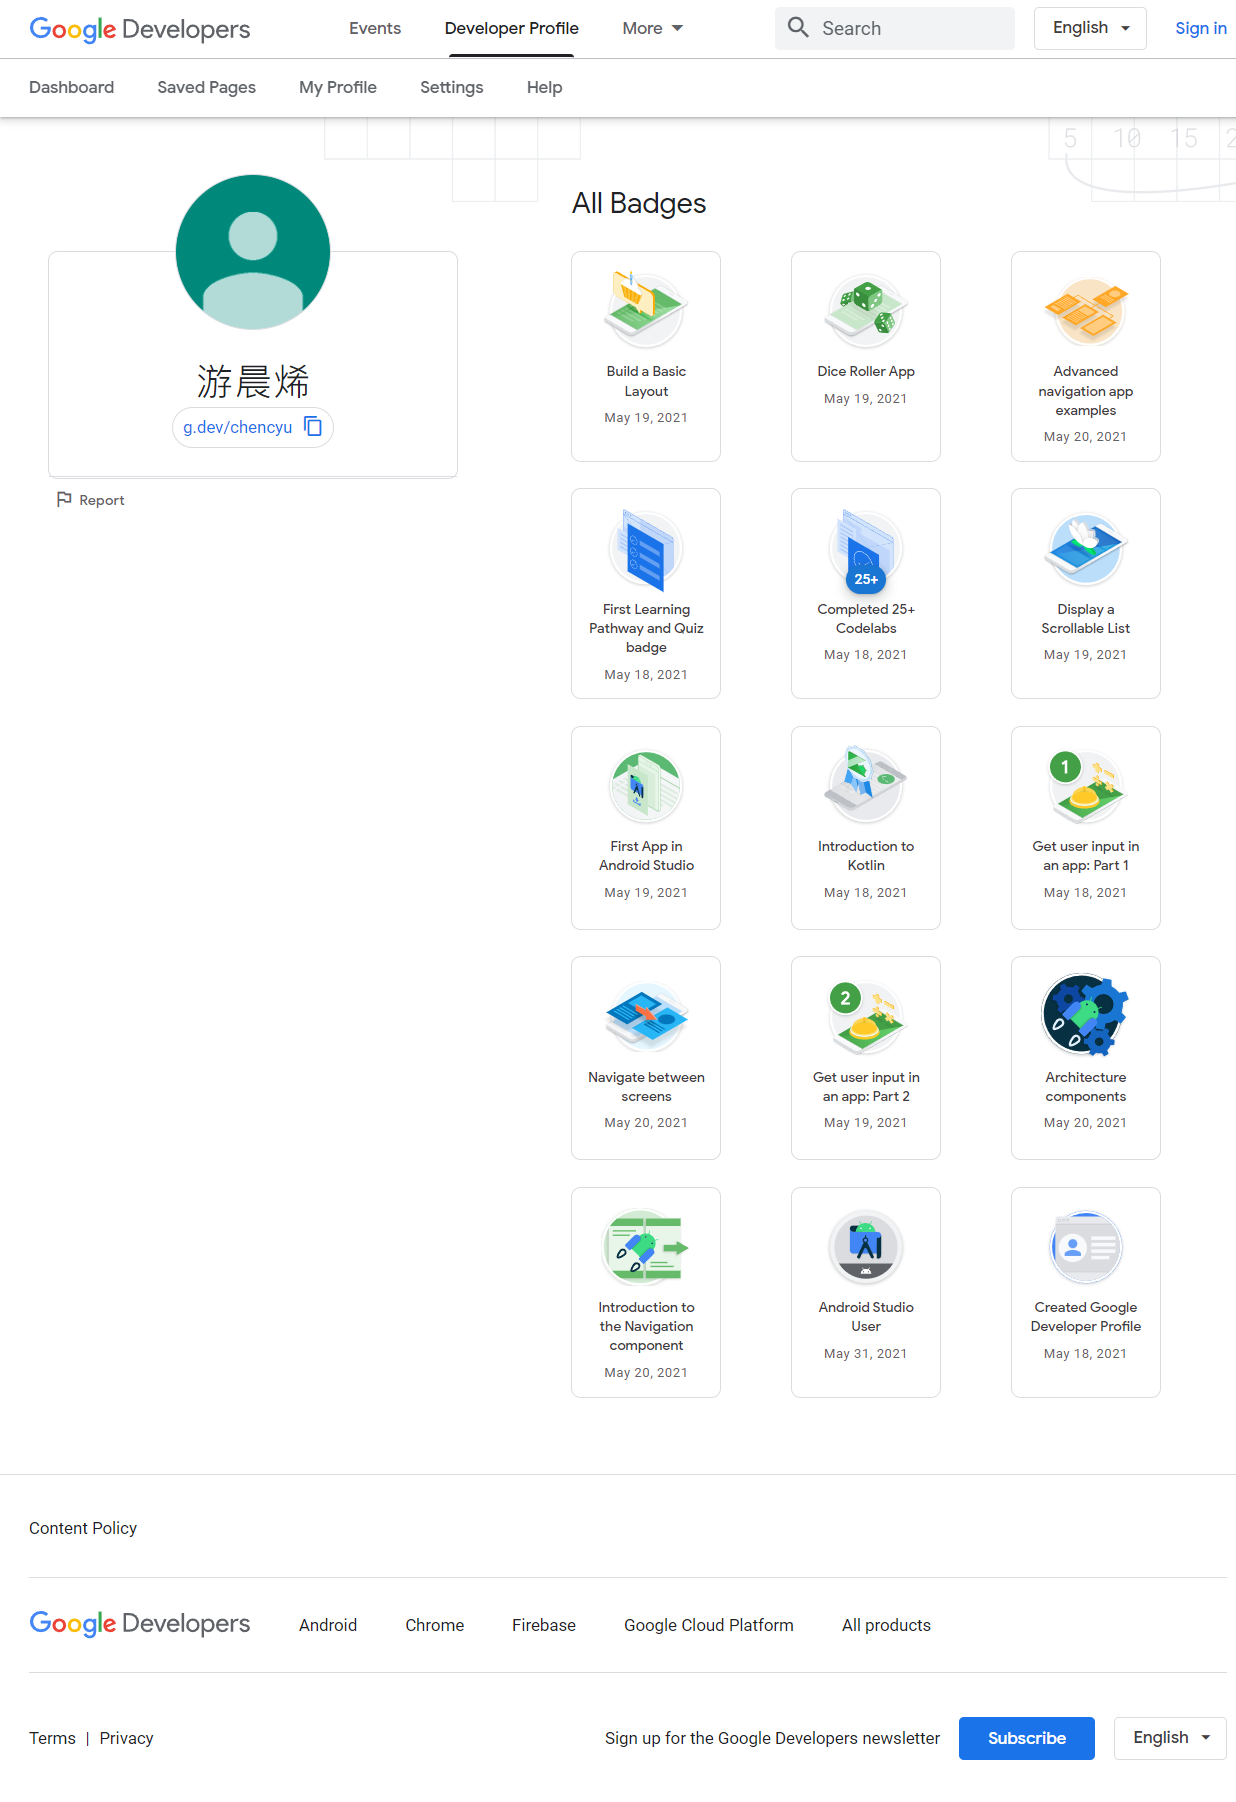
\includegraphics[scale=0.2, left]{android.png}}
    {\href{https://g.dev/chencyu}{\color{hyperlink}{Android Study Jam 2021(link)}}}
    {}{}{}

%---------------------------------------------------------
  \cventry
    {11 Badges\linebreak[1]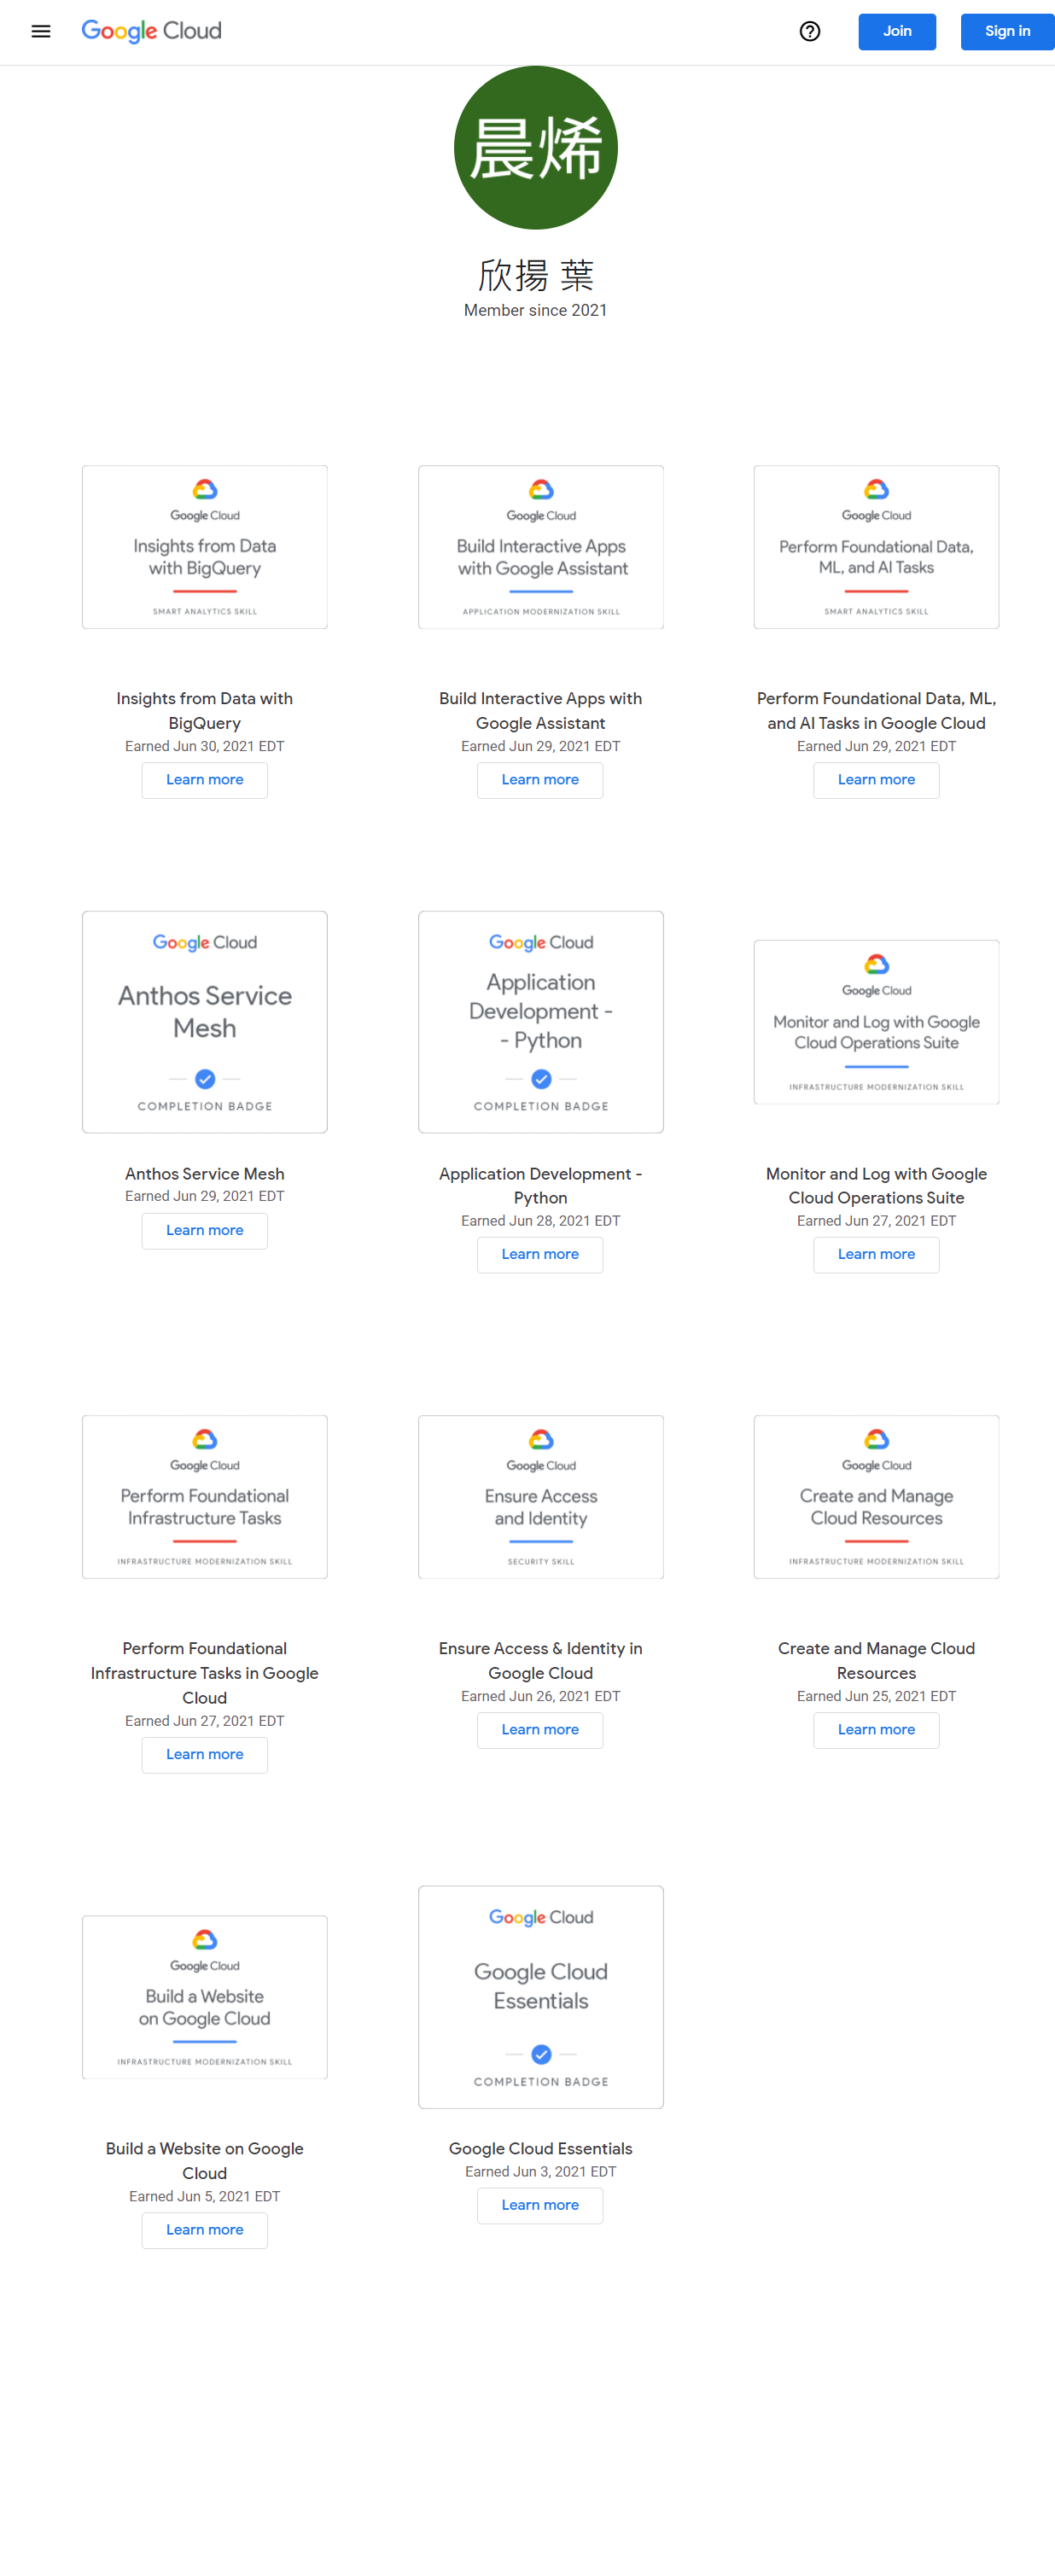
\includegraphics[scale=0.3, left]{gcp.png}}
    {\href{https://www.cloudskillsboost.google/public_profiles/1bfb275d-a0a0-4fa0-9c5c-3aa34a697132}{\color{hyperlink}{Google Cloud Jam 2021(link)}}}
    {}{}{}

%---------------------------------------------------------
  \cventry
    {via Mudras Identifier\linebreak[1]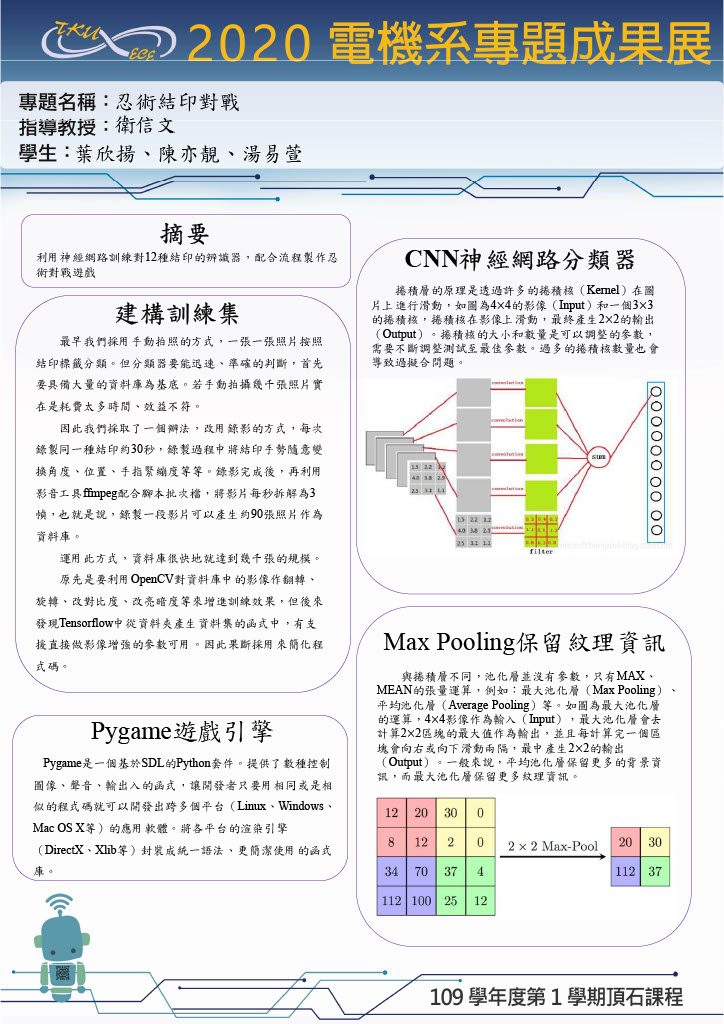
\includegraphics[scale=0.2, left]{naruto-battle.jpg}}
    {\href{https://github.com/chencyutku/Naruto-Battle-GUI}{\color{hyperlink}{Naruto-Battle game(link)}}}
    {}{}{}

%---------------------------------------------------------
  \cventry
    {via time-variant light \& caculating unlock alarm\linebreak[1]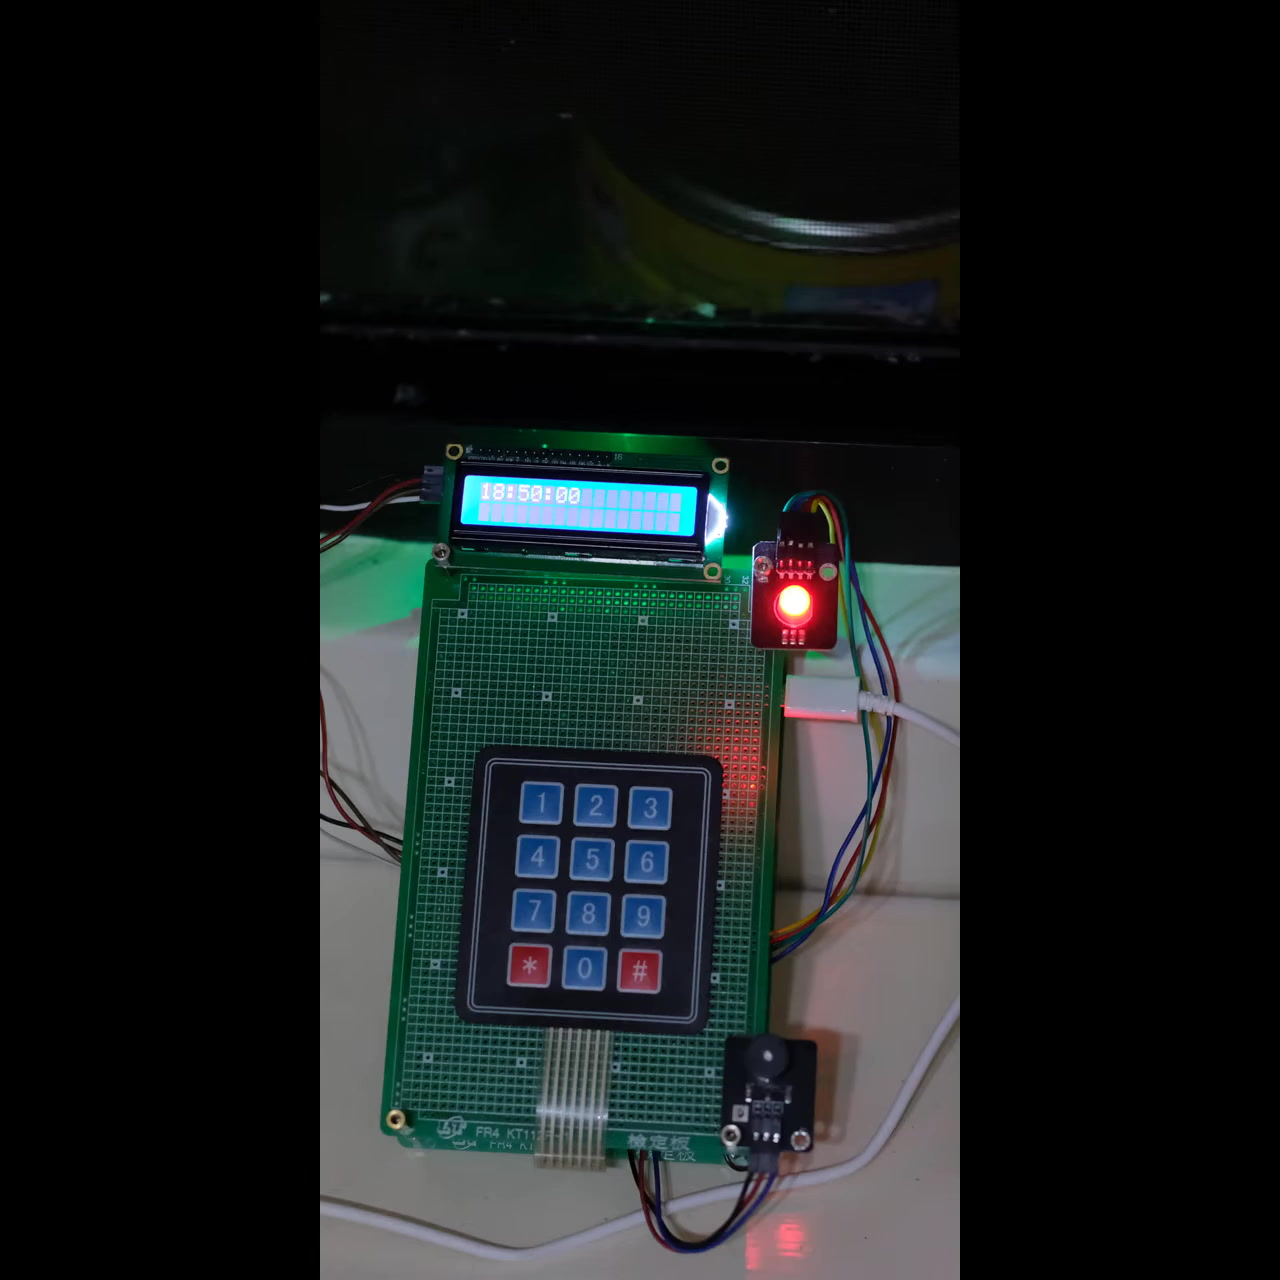
\includegraphics[scale=0.2, left]{refreshing-clock.jpg}}
    {\href{https://github.com/chencyutku/refreshing-clock}{\color{hyperlink}{Refreshin Clock(link)}}}
    {}{}{}

%---------------------------------------------------------
\end{cventries}

%\input{cv/honors.tex}
%\input{cv/presentation.tex}
%\input{cv/writing.tex}
%\input{cv/committees.tex}


%-------------------------------------------------------------------------------
\end{document}
